% ======================================================================
\section{Under what circumstances does SGDM converge?}\label{sec:circumstances}
% ======================================================================

The theorems of \cref{sec:convergence} hold under explicit \emph{sufficient} conditions.
This section asks which parts of these conditions can be removed, what goes wrong when
they fail, and how they fit together. Quadratic functions, for which everything can be
computed exactly, serve as test cases.

\subsection{A constant step size leaves a noise floor}

All constant-step results contain a term proportional to $\gamma\sigma^2$ that does not
vanish as $K\to\infty$. The next proposition shows that this is not an artifact of the
proofs: the floor is real, of exactly this order, and the same for SGD and SGDM at equal
effective step size.

\begin{proposition}[Exact noise floor on a quadratic]\label{prop:noise-floor}
Let $f(x)=\frac h2x^2$ on $\R$ with $h>0$, and let $g_k=hx_k+\xi_k$, where
$\xi_0,\xi_1,\dots$ are independent with $\E\xi_k=0$ and $\E\xi_k^2=\sigma^2$ (so
\cref{as:smooth,as:lower,as:unbiased,as:variance} hold with $L=h$). Let $\beta\in[0,1)$ and
$0<\alpha h<2(1+\beta)$. Then, for every starting point $x_0$,
\begin{equation}\label{eq:noise-floor}
  \lim_{k\to\infty}\E f(x_k)=\frac{\gamma\sigma^2}{2}\cdot\frac{1+\beta}{2(1+\beta)-\alpha h},
  \qquad
  \lim_{k\to\infty}\E\bigl[f'(x_k)^2\bigr]=h\gamma\sigma^2\cdot\frac{1+\beta}{2(1+\beta)-\alpha h}.
\end{equation}
In particular $\lim_k\E f(x_k)\ge\frac{\gamma\sigma^2}{4}$, and
$\lim_k\E f(x_k)=\frac{\gamma\sigma^2}{4}+\frac{\gamma\sigma^2}{4}\cdot\frac{\alpha h}{2(1+\beta)-\alpha h}$,
so to first order the floor depends on $(\alpha,\beta)$ only through $\gamma=\alpha/(1-\beta)$.
\end{proposition}

\begin{proof}
Let $a:=1+\beta-\alpha h$; the update reads $x_{k+1}=ax_k-\beta x_{k-1}-\alpha\xi_k$. With
$X_k:=(x_k,x_{k-1})^\top$ (and $x_{-1}=x_0$),
\[
  X_{k+1}=MX_k+w_k,\qquad M:=\begin{pmatrix}a&-\beta\\1&0\end{pmatrix},\qquad
  w_k:=\begin{pmatrix}-\alpha\xi_k\\0\end{pmatrix}.
\]
\emph{Second moments.} Let $C_k:=\E[X_kX_k^\top]$, a symmetric $2\times2$ matrix whose
$(1,1)$ entry is $\E x_k^2$. Since $X_k$ is a function of $\xi_0,\dots,\xi_{k-1}$, it is
independent of $\xi_k$, so $\E[X_kw_k^\top]=\E[X_k]\,\E[w_k]^\top=0$. Expanding the product,
\[
  C_{k+1}=\E\bigl[(MX_k+w_k)(MX_k+w_k)^\top\bigr]=MC_kM^\top+Q,\qquad
  Q:=\E[w_kw_k^\top]=\begin{pmatrix}\alpha^2\sigma^2&0\\0&0\end{pmatrix},
\]
and by induction $C_k=M^kC_0(M^\top)^k+\sum_{j=0}^{k-1}M^jQ(M^\top)^j$.

\emph{Convergence.} The eigenvalues of $M$ are the roots of
$\det(\lambda I-M)=\lambda^2-a\lambda+\beta$. By the proof of
\cref{prop:quadratic-stability} below, the assumption $0<\alpha h<2(1+\beta)$ implies that
both roots have modulus less than one. Then the entries of $M^k$ tend to zero
geometrically fast (\cref{lem:matrix-powers} in the appendix), so
$M^kC_0(M^\top)^k\to0$ and the series converges: $C_k\to C_\infty:=\sum_{j\ge0}M^jQ(M^\top)^j$.
Passing to the limit in the recursion, $C_\infty=MC_\infty M^\top+Q$.

\emph{Solving for the limit.} Write $C_\infty=\begin{pmatrix}s&r\\r&t\end{pmatrix}$. The
second row of $M$ is $(1,0)$ and the first is $(a,-\beta)$, so comparing entries of
$C_\infty=MC_\infty M^\top+Q$ gives
\[
  (2,2):\ t=s;\qquad (1,2):\ r=as-\beta r;\qquad (1,1):\ s=a^2s-2a\beta r+\beta^2t+\alpha^2\sigma^2 .
\]
Hence $r=\frac{as}{1+\beta}$, and substituting into the $(1,1)$ equation and multiplying by
$1+\beta$:
$s\bigl[(1+\beta)(1-\beta^2)-a^2(1+\beta)+2a^2\beta\bigr]=\alpha^2\sigma^2(1+\beta)$. The
bracket equals $(1+\beta)(1-\beta^2)-a^2(1-\beta)=(1-\beta)\bigl[(1+\beta)^2-a^2\bigr]$, and
$(1+\beta)^2-a^2=(1+\beta-a)(1+\beta+a)=\alpha h\,\bigl(2(1+\beta)-\alpha h\bigr)$. Therefore
\[
  s=\frac{\alpha^2\sigma^2(1+\beta)}{(1-\beta)\,\alpha h\,(2(1+\beta)-\alpha h)}
   =\frac{\gamma\sigma^2}{h}\cdot\frac{1+\beta}{2(1+\beta)-\alpha h}.
\]
Since $\E f(x_k)=\frac h2\E x_k^2\to\frac h2 s$ and $\E f'(x_k)^2=h^2\E x_k^2\to h^2s$, we
obtain \eqref{eq:noise-floor}. Finally,
$\frac{1+\beta}{2(1+\beta)-\alpha h}=\frac12+\frac{\alpha h}{2(2(1+\beta)-\alpha h)}\ge\frac12$.
\end{proof}

\paragraph{Consequences.}
(i) With a constant step and $\sigma>0$, $\E f(x_k)$ does not converge to $\fs$; the floor is
of order $\gamma\sigma^2$, exactly as in \cref{thm:nonconvex,thm:pl}. With $L=h$,
\eqref{eq:noise-floor} gives $\lim_k\E f'(x_k)^2\approx\frac{L\gamma\sigma^2}{2}$, while
\cref{thm:nonconvex} guarantees at most $4L\gamma\sigma^2$: the theorem is pessimistic only by
a constant factor. (ii) At equal \emph{effective} step size, SGD ($\beta=0$) and SGDM have the
same floor to first order: momentum does not average the noise away. At equal \emph{raw}
step $\alpha$, momentum raises the floor by the factor $1/(1-\beta)$. (iii) To converge
exactly, one must let the step size decrease (\cref{thm:diminishing,cor:pl-decay}), reduce
the variance (larger mini-batches, \cref{rem:minibatch}), or have exact gradients
(\cref{cor:deterministic}). \Cref{fig:noise-floor} confirms \eqref{eq:noise-floor}
numerically.

\subsection{Too large a step size: the exact stability region on quadratics}

\begin{proposition}[Heavy ball on a quadratic]\label{prop:quadratic-stability}
Let $f(x)=\frac h2x^2$ with $h>0$, exact gradients, $\beta\in[0,1)$ and $\alpha>0$. The
heavy-ball iteration $x_{k+1}=(1+\beta-\alpha h)x_k-\beta x_{k-1}$ converges to $0$ for
every initial pair $(x_{-1},x_0)$ if and only if
\begin{equation}\label{eq:stability}
  \alpha h<2(1+\beta).
\end{equation}
In that case the convergence is linear with rate $\max\{|\lambda_1|,|\lambda_2|\}<1$,
where $\lambda_{1,2}$ are the roots of $p(\lambda)=\lambda^2-(1+\beta-\alpha h)\lambda+\beta$.
For $f(x)=\frac12x^\top Hx$ with $H$ symmetric positive definite with largest eigenvalue
$L$, the iteration converges for all initial conditions if and only if $\alpha L<2(1+\beta)$.
\end{proposition}

\begin{proof}
Let $a=1+\beta-\alpha h$. By \cref{lem:recurrence} in the appendix, every solution of
$x_{k+1}=ax_k-\beta x_{k-1}$ has the form $c_1\lambda_1^k+c_2\lambda_2^k$ (distinct roots)
or $(c_1+c_2k)\lambda_1^k$ (double root), and every such sequence is a solution. Hence all
solutions tend to $0$ if both roots satisfy $|\lambda_i|<1$; and if some root has
$|\lambda_1|\ge1$ and is real, the solution with $x_{-1}=1$, $x_0=\lambda_1$, namely
$x_k=\lambda_1^{k+1}$, does not tend to $0$. It remains to relate the roots to
\eqref{eq:stability}.

\emph{If \eqref{eq:stability} holds, both roots have modulus $<1$.} If the roots are complex
($a^2<4\beta$), they are conjugate, and $|\lambda_1|^2=\lambda_1\lambda_2=\beta<1$. If they are
real ($a^2\ge4\beta$), observe that $p(1)=1-a+\beta=\alpha h>0$ and
$p(-1)=1+a+\beta=2(1+\beta)-\alpha h>0$. Since $p$ is an upward parabola, $p\le0$ on the
interval $[\lambda_1,\lambda_2]$ between its roots, so neither $1$ nor $-1$ belongs to this
interval; it therefore lies entirely in $(-\infty,-1)$, in $(-1,1)$, or in $(1,\infty)$.
In the first and third cases $|\lambda_1\lambda_2|>1$, contradicting $\lambda_1\lambda_2=\beta<1$.
Hence both roots lie in $(-1,1)$.

\emph{If \eqref{eq:stability} fails, some root is real with modulus $\ge1$.} Then
$p(-1)=2(1+\beta)-\alpha h\le0$, and since $p(\lambda)\to+\infty$ as $\lambda\to-\infty$,
the intermediate value theorem gives a real root $\lambda\le-1$.

For the matrix case, diagonalize $H=U\Lambda U^\top$ with $U$ orthogonal. In the coordinates
$y=U^\top x$ the iteration decouples into $d$ scalar iterations with $h=\Lambda_{ii}$, and all
of them converge for all initial conditions if and only if $\alpha\Lambda_{ii}<2(1+\beta)$
for every $i$, i.e.\ $\alpha L<2(1+\beta)$.
\end{proof}

\paragraph{Momentum on quadratics.} For gradient descent ($\beta=0$) the condition is the
familiar $\alpha L<2$. Momentum enlarges it to $\alpha L<2(1+\beta)$, or, in terms of the
effective step, $\gamma L<\frac{2(1+\beta)}{1-\beta}$, which equals $38$ for $\beta=0.9$. On
quadratics momentum can also accelerate: if the eigenvalues of $H$ lie in $[\mu,L]$ and
$\kappa=L/\mu$, Polyak's choice~\cite{polyak1964}
$\alpha=\frac{4}{(\sqrt L+\sqrt\mu)^2}$, $\beta=\bigl(\frac{\sqrt L-\sqrt\mu}{\sqrt L+\sqrt\mu}\bigr)^2$
gives $(1-\sqrt\beta)^2=\alpha\mu$ and $(1+\sqrt\beta)^2=\alpha L$, so for every eigenvalue
$h\in[\mu,L]$ we have $|1+\beta-\alpha h|\le2\sqrt\beta$; the roots are then complex (or
double) with modulus $\sqrt\beta=\frac{\sqrt\kappa-1}{\sqrt\kappa+1}$, compared with the
rate $\frac{\kappa-1}{\kappa+1}$ of optimally tuned gradient descent. Both facts are special
to quadratics with exact gradients: \cref{ex:lrp} below shows that the same parameters can
fail on a smooth strongly convex function, and \cref{prop:noise-floor} shows that with
noise the floor is governed by $\gamma$.

\subsection{Without noise, larger steps are safe for every smooth function}

\begin{proposition}[Mechanical energy decreases]\label{prop:energy}
Let \cref{as:smooth,as:lower} hold, use exact gradients ($g_k=\nabla f(x_k)$),
$\beta\in[0,1)$ and $0<\alpha<\frac{2(1-\beta)}{L}$. Let
$V_k:=f(x_k)+\frac{\beta}{2\alpha}\norm{x_k-x_{k-1}}^2$. Then for all $k\ge0$,
\begin{equation}\label{eq:energy}
  V_{k+1}\le V_k-\Bigl(\frac{1-\beta}{\alpha}-\frac L2\Bigr)\norm{x_{k+1}-x_k}^2,
\end{equation}
and $\min_{0\le k<K}\norm{\nabla f(x_k)}^2\le\frac{2(1+\beta^2)\Dlt}{\alpha\,(1-\beta-\alpha L/2)\,K}$.
In particular $\nabla f(x_k)\to0$.
\end{proposition}

\begin{proof}
With $v_k=x_k-x_{k-1}$, the update gives $\alpha\nabla f(x_k)=\beta v_k-v_{k+1}$. The descent
lemma with $x=x_k$, $y=x_{k+1}$ and Young's inequality ($\rho=1$) give
\[
  f(x_{k+1})\le f(x_k)+\frac1\alpha\bigl(\beta\ip{v_k}{v_{k+1}}-\norm{v_{k+1}}^2\bigr)+\frac L2\norm{v_{k+1}}^2
  \le f(x_k)+\frac\beta{2\alpha}\norm{v_k}^2+\Bigl(\frac\beta{2\alpha}-\frac1\alpha+\frac L2\Bigr)\norm{v_{k+1}}^2 .
\]
Adding $\frac{\beta}{2\alpha}\norm{v_{k+1}}^2$ to both sides gives \eqref{eq:energy}. The
coefficient $c:=\frac{1-\beta}\alpha-\frac L2$ is positive by assumption. Summing
\eqref{eq:energy} and using $V_0=f(x_0)$ (as $v_0=0$) and $V_K\ge\fs$,
$\sum_{j=1}^K\norm{v_j}^2\le\Dlt/c$. Finally
$\norm{\nabla f(x_k)}^2=\alpha^{-2}\norm{\beta v_k-v_{k+1}}^2\le2\alpha^{-2}(\beta^2\norm{v_k}^2+\norm{v_{k+1}}^2)$
by \cref{lem:elementary}(e); summing over $k<K$ and using $v_0=0$,
$\sum_{k<K}\norm{\nabla f(x_k)}^2\le\frac{2(1+\beta^2)}{\alpha^2}\sum_{j=1}^K\norm{v_j}^2
\le\frac{2(1+\beta^2)\Dlt}{\alpha^2c}$, and $\alpha^2c=\alpha(1-\beta-\alpha L/2)$.
The minimum is at most the average.
\end{proof}

This ``kinetic plus potential energy'' argument is classical~\cite{zavriev1993}; see
also~\cite{ghadimi2015} for the convex case. The condition $\alpha<\frac{2(1-\beta)}L$ reads
$\gamma<\frac2L$: exactly the step-size range of gradient descent. So \emph{without noise},
heavy ball is safe for every smooth function as long as its effective step is a safe
gradient-descent step.

\begin{remark}[Why the energy argument fails with noise]\label{rem:energy-noise}
With $g_k=\nabla f(x_k)+\eps_k$, the same computation gives
$V_{k+1}\le V_k-c\norm{v_{k+1}}^2-\ip{\eps_k}{v_{k+1}}$. Since
$v_{k+1}=(\beta v_k-\alpha\nabla f(x_k))-\alpha\eps_k$, we get
$\Ek\ip{\eps_k}{v_{k+1}}=-\alpha\Ek\norm{\eps_k}^2$ and
$\Ek\norm{v_{k+1}}^2=\norm{\beta v_k-\alpha\nabla f(x_k)}^2+\alpha^2\Ek\norm{\eps_k}^2$, hence
\[
  \Ek V_{k+1}\le V_k-c\,\norm{\beta v_k-\alpha\nabla f(x_k)}^2+\alpha\Bigl(\beta+\frac{\alpha L}{2}\Bigr)\Ek\norm{\eps_k}^2 .
\]
For $\beta=0$ the noise term is the SGD term $\frac{L\alpha^2}2\sigma^2$, but for $\beta>0$ it
is of \emph{first} order in $\alpha$. Telescoped over $K$ steps it contributes $K\alpha\beta\sigma^2$,
which is of the same order as the total progress, and the resulting bound does not vanish
as $\alpha\to0$. The potential $\Phi_k$ of \cref{thm:master} pays only $L\gamma^2\sigma^2$
per step; this is why the stochastic analysis is built on the extrapolated point.
\end{remark}

\subsection{Quadratic intuition can mislead: a counterexample}

\begin{example}[Lessard--Recht--Packard~\cite{lessard2016}]\label{ex:lrp}
Consider the piecewise quadratic function
\[
  f(x)=\begin{cases}\frac{25}{2}x^2, & x<1,\\[2pt] \frac12x^2+24x-12, & 1\le x<2,\\[2pt]
  \frac{25}{2}x^2-24x+36, & x\ge2,\end{cases}
  \qquad
  f'(x)=\begin{cases}25x, & x<1,\\ x+24, & 1\le x<2,\\ 25x-24, & x\ge2.\end{cases}
\]
One checks that $f$ and $f'$ are continuous at $x=1$ and $x=2$, and that $f''\in\{1,25\}$
away from these points, so $f$ is $1$-strongly convex and $25$-smooth with minimizer
$x^\star=0$. Take Polyak's quadratic-optimal parameters for $\mu=1$, $L=25$:
$\alpha=\frac{4}{(5+1)^2}=\frac19$ and $\beta=\bigl(\frac{5-1}{5+1}\bigr)^2=\frac49$. These
satisfy \eqref{eq:stability} ($\alpha L=\frac{25}9<\frac{26}{9}=2(1+\beta)$), so on \emph{every}
quadratic with curvature in $[1,25]$ heavy ball converges, at rate $\frac23$.

On $f$, however, it does not. With these parameters the update reads
$x_{k+1}=\frac{13}9x_k-\frac49x_{k-1}-\frac19f'(x_k)$, that is,
\[
  x_{k+1}=-\tfrac43x_k-\tfrac49x_{k-1}\quad\text{if }x_k<1,\qquad
  x_{k+1}=-\tfrac43x_k-\tfrac49x_{k-1}+\tfrac83\quad\text{if }x_k\ge2 .
\]
Let $p_1=\frac{792}{1225}\approx0.647$, $p_2=-\frac{2208}{1225}\approx-1.802$ and
$p_3=\frac{2592}{1225}\approx2.116$. Starting from $(x_{k-1},x_k)=(p_3,p_1)$:
\begin{align*}
  p_1<1:&\quad -\tfrac43\cdot\tfrac{792}{1225}-\tfrac49\cdot\tfrac{2592}{1225}=\tfrac{-1056-1152}{1225}=p_2,\\
  p_2<1:&\quad -\tfrac43\cdot\bigl(-\tfrac{2208}{1225}\bigr)-\tfrac49\cdot\tfrac{792}{1225}=\tfrac{2944-352}{1225}=p_3,\\
  p_3\ge2:&\quad -\tfrac43\cdot\tfrac{2592}{1225}-\tfrac49\cdot\bigl(-\tfrac{2208}{1225}\bigr)+\tfrac83
           =\tfrac{-31104+8832+29400}{11025}=\tfrac{7128}{11025}=p_1 .
\end{align*}
So $p_1\to p_2\to p_3\to p_1\to\cdots$ is a periodic orbit: from $x_{-1}=p_3$, $x_0=p_1$ the
iterates cycle forever and $f(x_k)\ge f(p_1)\approx5.2$ for all $k$, although $f$ is
strongly convex and smooth. Moreover the cycle attracts nearby trajectories: from
$x_{-1}=x_0=3.3$ the iterates converge to it (\cref{fig:lrp}; \cite{lessard2016} reports
this for all $x_0=x_{-1}\in[3.07,3.46]$).
\end{example}

The parameters of \cref{ex:lrp} lie inside the quadratic stability region but violate all of
our conditions: $\alpha=\frac19$ exceeds $\frac{2(1-\beta)}{L}=\frac2{45}$ (\cref{prop:energy}),
$\frac{1-\beta}{2L}=\frac1{90}$ (\cref{thm:convex}) and $\frac{(1-\beta)^2}{2L}=\frac1{162}$
(\cref{thm:master}). With $\beta=\frac49$ and $\alpha=0.04<\frac2{45}$ or
$\alpha=\frac1{162}$, the same function and starting point give fast convergence
(\cref{fig:lrp}).

\begin{figure}[t]
\centering
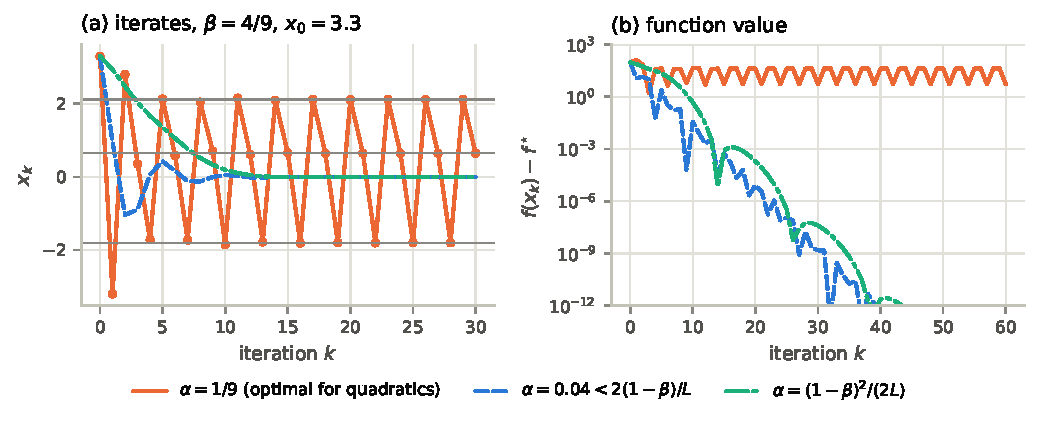
\includegraphics[width=\textwidth]{figures/counterexample.pdf}
\caption{Heavy ball on the strongly convex function of \cref{ex:lrp}, $\beta=\frac49$,
$x_{-1}=x_0=3.3$, exact gradients. (a)~With the quadratic-optimal $\alpha=\frac19$ the iterates
are attracted to the $3$-cycle $\{p_1,p_2,p_3\}$ (grey lines). (b)~The function value then
oscillates forever, while the step sizes allowed by \cref{prop:energy} ($\alpha=0.04$) and by
\cref{thm:master} ($\alpha=(1-\beta)^2/(2L)$) converge.}
\label{fig:lrp}
\end{figure}

\subsection{The map of the parameter plane}\label{sec:map}

\Cref{fig:regions} collects the step-size conditions as regions in the $(\beta,\alpha)$
plane, nested from the most special setting to the most general one:
\begin{itemize}
\item[R4] quadratic $f$, exact gradients: convergence if and only if $\alpha L<2(1+\beta)$
          (\cref{prop:quadratic-stability});
\item[R3] any $L$-smooth $f$, exact gradients: $\alpha L<2(1-\beta)$ suffices
          (\cref{prop:energy});
\item[R2] convex $f$, stochastic gradients: $\alpha L\le\frac{1-\beta}{2}$ suffices
          (\cref{thm:convex});
\item[R1] nonconvex $f$, stochastic gradients: $\alpha L\le\frac{(1-\beta)^2}{2}$ suffices
          (\cref{thm:master,thm:nonconvex}).
\end{itemize}
Panel (b) shows the same regions in terms of the effective step size. There the picture is
strikingly simple: R3 is $\gamma L<2$ and R2 is $\gamma L\le\frac12$, both independent of
$\beta$---momentum with effective step $\gamma$ is as safe as gradient descent with step
$\gamma$---whereas R1 shrinks like $\gamma L\le\frac{1-\beta}{2}$, and R4 (quadratics) grows
without bound as $\beta\to1$. The star (\cref{ex:lrp}) lies in R4 but outside R3, and the
method indeed fails there.

We stress that R1--R3 are \emph{sufficient} conditions. In particular we do not claim that
R1 is necessary for stochastic nonconvex problems; it is the price of a short, general
proof, and in practice larger steps are often used successfully. What the figure does show
is that the question ``does SGDM converge?'' has different answers for different function
classes, and that conclusions drawn from quadratics (R4) do not transfer to general
functions.

\begin{figure}[t]
\centering
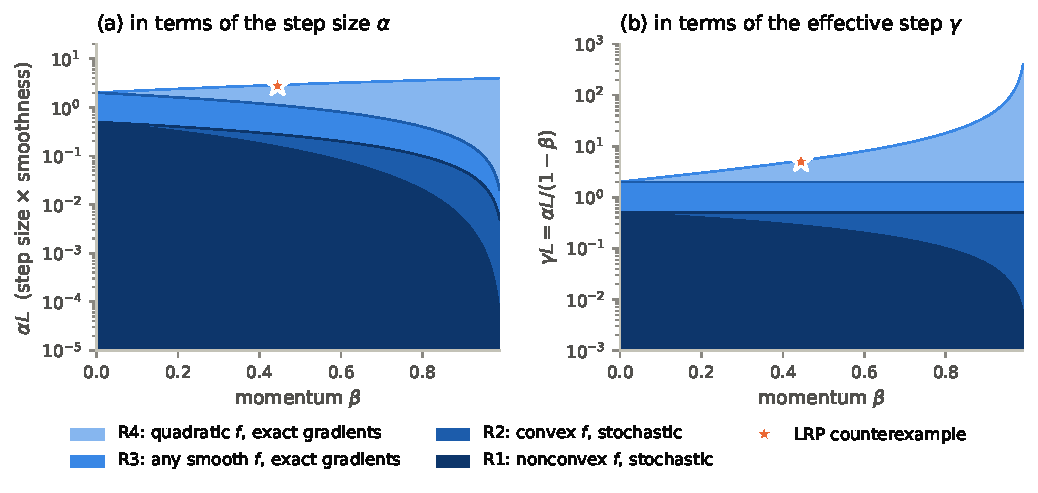
\includegraphics[width=\textwidth]{figures/regions.pdf}
\caption{Where each guarantee holds. Nested regions of admissible parameters,
(a)~in terms of $\alpha L$, (b)~in terms of the effective step $\gamma L=\alpha L/(1-\beta)$
(log scales). R1: \cref{thm:master} (nonconvex, stochastic); R2: \cref{thm:convex}
(convex, stochastic); R3: \cref{prop:energy} (any smooth $f$, exact gradients); R4:
\cref{prop:quadratic-stability} (quadratics, exact gradients). The star marks the
parameters of \cref{ex:lrp}, for which heavy ball cycles on a strongly convex function.}
\label{fig:regions}
\end{figure}

\subsection{Does momentum help?}\label{sec:momentum-help}

The results above give a nuanced answer.
\begin{itemize}
\item \emph{At equal effective step size, SGDM behaves like SGD.} The bounds of
  \cref{sec:convergence} coincide with the SGD bounds up to constants when $\alpha$ is replaced
  by $\gamma$; the noise floor is the same to first order (\cref{prop:noise-floor}); and in
  experiments the trajectories are nearly indistinguishable (\cref{fig:sgd-vs-sgdm}(a)).
  This matches the conclusion of~\cite{liu2020} that SGDM converges as fast as SGD.
\item \emph{At equal raw step size, momentum is a larger step.} It multiplies the effective
  step by $1/(1-\beta)$: faster initial progress, but a floor that is $1/(1-\beta)$ times
  higher (\cref{fig:sgd-vs-sgdm}(b)). Increasing $\beta$ without decreasing $\alpha$ is
  therefore not ``free''.
\item \emph{No worst-case acceleration.} In our analysis the admissible effective step shrinks
  as $\beta\to1$ (R1), and the PL rate $1-\frac{\gamma\mu}{4}$ is no better than that of SGD.
  Acceleration (\cref{sec:circumstances}, ``Momentum on quadratics'') relies on quadratic
  structure and exact gradients; it fails for general strongly convex functions
  (\cref{ex:lrp}) and, for stochastic gradients, there are problems on which the stochastic
  heavy-ball method provably does not improve on SGD~\cite{kidambi2018}.
\end{itemize}
The practical popularity of momentum is therefore better explained by its behaviour on
problems that are locally close to quadratic and ill-conditioned, where the gradient noise
is small relative to the signal, than by worst-case guarantees.

\subsection{When the assumptions fail}

\begin{itemize}
\item \emph{$\beta\ge1$ (no friction).} The roots of $p$ in \cref{prop:quadratic-stability}
  have product $\beta\ge1$, so at least one has modulus $\ge1$: heavy ball does not converge
  even on $\frac12x^2$. The extrapolated point and the effective step size are undefined.
  The condition $\beta<1$ is necessary.
\item \emph{Noise growing with the gradient},
  $\Ek\norm{g_k-\nabla f(x_k)}^2\le\sigma^2+M\norm{\nabla f(x_k)}^2$: all results remain
  valid with the step-size condition tightened by the factor $1+M$
  (\cref{rem:extensions}(ii)).
\item \emph{Infinite variance (heavy-tailed noise).} \Cref{as:variance} fails and the bounds
  above are vacuous; techniques such as gradient clipping are then used. This is beyond the
  scope of this report.
\item \emph{Biased gradients.} Unbiasedness (\cref{as:unbiased}) is used in
  \cref{lem:z-descent,lem:velocity}. With a bias, both lemmas acquire additional error
  terms and convergence can only be guaranteed up to a neighbourhood whose size depends on
  the bias.
\item \emph{Non-smooth $f$.} Without \cref{as:smooth} there is no descent lemma; momentum
  methods for non-smooth (weakly convex) problems require different tools,
  see~\cite{mai2020}.
\end{itemize}

\subsection{Summary: a checklist}

SGDM achieves the SGD-style expected decrease, and hence the convergence guarantees of
\cref{sec:convergence}, under the following circumstances.
\begin{enumerate}
\item \textbf{The problem:} $f$ is $L$-smooth and bounded below; the stochastic gradients are
  unbiased with bounded variance $\sigma^2$ (\cref{as:smooth,as:lower,as:unbiased,as:variance}).
\item \textbf{The momentum:} $\beta\in[0,1)$---friction must be present.
\item \textbf{The step size, measured as the effective step $\gamma=\alpha/(1-\beta)$:}
  \begin{itemize}
  \item general nonconvex, stochastic: $\gamma\le\frac{1-\beta}{2L}$, i.e.\ $\alpha\le\frac{(1-\beta)^2}{2L}$;
  \item convex, stochastic: $\gamma\le\frac{1}{2L}$;
  \item any smooth $f$, exact gradients: $\gamma<\frac2L$.
  \end{itemize}
\item \textbf{The target:} with a constant step one reaches a noise region of size
  $O(\gamma\sigma^2)$, which is unavoidable (\cref{prop:noise-floor}); to reach accuracy
  $\eps^2$ in $\min_k\E\norm{\nabla f(x_k)}^2$ choose $\gamma\propto1/\sqrt K$
  (\cref{cor:rate}), or use decaying steps (\cref{thm:diminishing}) for asymptotic convergence.
\item \textbf{Linear rates} need additional structure such as the PL inequality or strong
  convexity (\cref{thm:pl}); the rate is $1-\gamma\mu/4$.
\item \textbf{Beware of quadratic intuition:} parameters that are stable or even optimal for
  quadratics can make the method cycle on a strongly convex function (\cref{ex:lrp}).
\end{enumerate}
